\section{Results}
\subsection{Length fitting leaves condition-dependent shape discrepancy}
The one-target calibration reproduces the B length proxy while leaving a systematic width/depth residual at B and C (Table~\ref{tab:geometry} and Fig.~\ref{fig:comparison}). The fitted length is 359.16~\um, but the B width exceeds the nominal reference by 19.54~\um\ and depth falls below it by 4.88~\um. Their separate expanded-uncertainty-scale ratios are +3.10 and $-1.23$. Thus length fitting does not reproduce the remaining B shape quantities.

\begin{table}[htbp]
\centering
\caption{Condition-level geometry comparisons in \um. $U$ is the separately sourced Lane expanded uncertainty ($k=2$). Reference width/depth means are current NIST 100~\us-track classes. B length is fitted. $\delta/U$ uses only the experimental scale, without combined model uncertainty.}
\label{tab:geometry}
\small
\begin{tabular}{llrrrr}
\toprule
Condition & Quantity & Model & Reference & $U$ & $\delta/U$\\
\midrule
A & $L$ & 309.89 & 300 & 11.91 & +0.83\\
  & $W$ & 153.36 & 147.9 & 6.42 & +0.85\\
  & $D$ & 40.47 & 42.5 & 4.49 & $-0.45$\\
B & $L$ (fitted) & 359.16 & 359 & 21.26 & +0.01\\
  & $W$ & 143.04 & 123.5 & 6.30 & +3.10\\
  & $D$ & 31.12 & 36 & 3.97 & $-1.23$\\
C & $L$ & 320.63 & 370 & 32.57 & $-1.52$\\
  & $W$ & 129.05 & 106 & 4.48 & +5.14\\
  & $D$ & 22.04 & 29.6 & 3.26 & $-2.32$\\
\bottomrule
\end{tabular}
\end{table}

\begin{figure}[htbp]
\centering
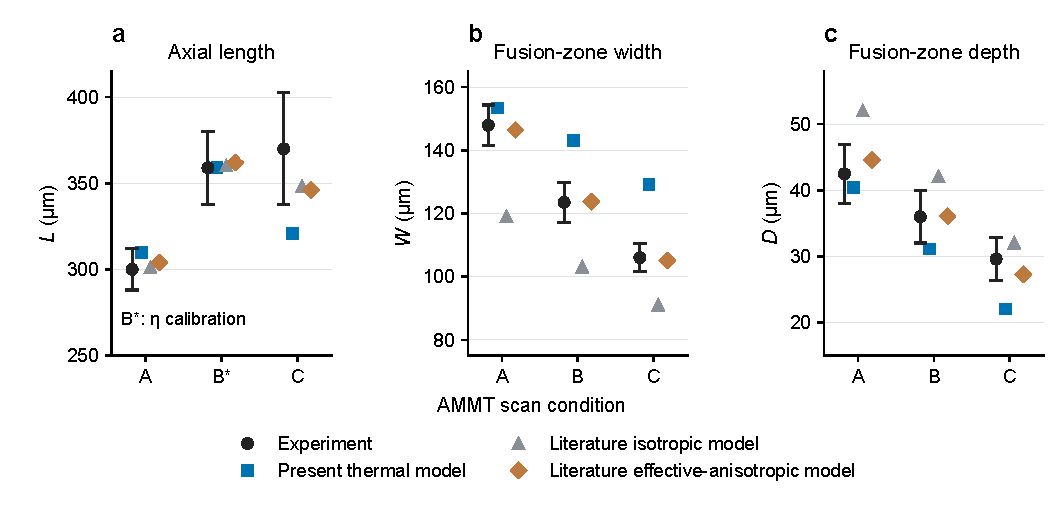
\includegraphics[width=\textwidth]{figures/ammt-application-experiment.pdf}
\caption{Geometry comparison with condition-level reference means and the published isotropic and effective-anisotropic calculations of Kollmannsberger et al.~\cite{kollmannsberger2019}. Experimental bars show separately sourced Lane $U(k=2)$ scales; width/depth centers use current NIST means. B length is calibrated in the present model. Published-model points provide context: beam representation, phase law, parameter calibration and observation definitions differ, so this is not a controlled ranking of solvers.}
\label{fig:comparison}
\end{figure}

A differences are smaller than their respective reported uncertainty scales. In C, the model is 49.37~\um\ shorter, 23.05~\um\ wider and 7.56~\um\ shallower than the nominal references. The wide/shallow pattern is also apparent in the predicted aspect ratios $W/D=3.79,4.60,5.85$ for A/B/C, compared with condition-level reference ratios 3.48,3.43,3.58. These ratios combine separate class means; they are not specimen-wise aspect-ratio measurements.

At fixed power from B to C, a 50\% speed increase reduces absorbed line energy by one third. Model width decreases by 9.78\% and depth by 29.16\%; the nominal reference changes are 14.17\% and 17.78\%. The modeled $W/D$ increases by 27.36\% from B to C. The shape discrepancy therefore concerns the relative contraction of transverse and depth extents as well as their absolute values. A--B changes cannot be attributed to speed alone because power also changes.

Nominal experimental length increases by 11~\um\ from B to C, whereas model length decreases by 38.53~\um. The 11~\um\ increase is smaller than the 38.89~\um\ zero-correlation quadrature of the two reported expanded-uncertainty scales. The data therefore do not establish a statistically resolved opposite experimental length trend. C's individual discrepancy remains distinct from that trend comparison. Retained axial changes below 0.37~\um\ are far smaller than the main B/C residuals; refining that direction alone is unlikely to remove the observed shape pattern.

\begin{figure}[htbp]
\centering
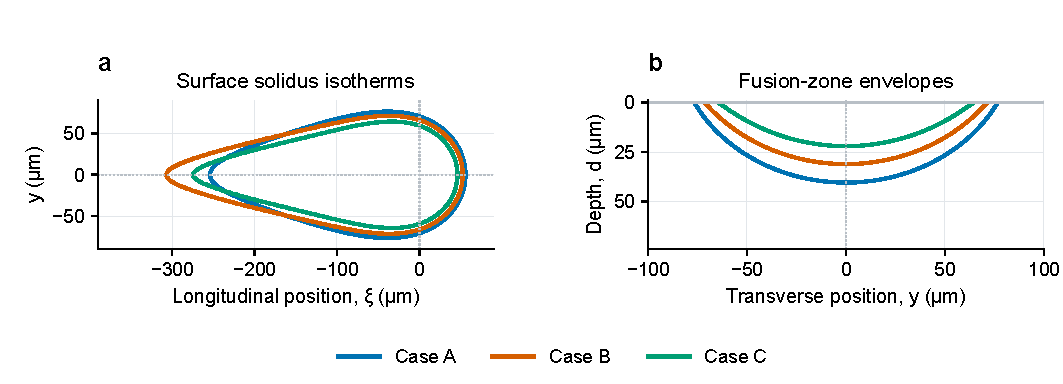
\includegraphics[width=\textwidth]{figures/ammt-research-operating-cases.pdf}
\caption{Model geometry for A, B and C. (a) Surface solidus contours in laser-frame coordinates. (b) Reconstructed maximum-temperature fusion envelopes in transverse/depth coordinates. Fusion envelopes use slice reconstruction and interpolation before passage maximization. The fields are model outputs, not microscopy or inferred liquid-flow maps. Both panels use the fixed calibrated source factor.}
\label{fig:fields}
\end{figure}

The common physical axes make the decrease in penetration relative to transverse width apparent. The surface contour and fusion envelope answer different geometric questions: the first determines the surface length proxy, while the second follows the maximum-temperature material passage through the field.

\subsection{Spatial phase span and material cooling time separate across speed}
The rear centerline phase spans are 48.30, 80.26 and 80.79~\um\ for A/B/C (Fig.~\ref{fig:trends}). The B/C spans differ by only 0.53~\um, yet their transformed passage times are 100.33 and 67.33~\us. The C span is 0.66\% larger, while the passage time is 32.90\% shorter because speed increases from 0.8 to 1.2~m/s. The corresponding interval-mean cooling rate rises from 0.598 to 0.891~\si{\mega\kelvin\per\second}; A gives 120.74~\us{} and 0.497~\si{\mega\kelvin\per\second}. Thus the B-to-C interval-mean cooling rate increases by 49.02\% despite only a 0.53~\um{} difference in the spatial phase span.

The result is a distinction between spatial structure and exposure time, rather than an independent cooling-rate validation. It follows directly from the coordinate relation in Eq.~\eqref{eq:passage}. A phase-span image alone cannot specify the material thermal interval without the scan speed. The inferred histories refer to the centerline and adopted equilibrium phase law; they do not predict grain morphology, segregation or final microstructure.

\begin{figure}[htbp]
\centering
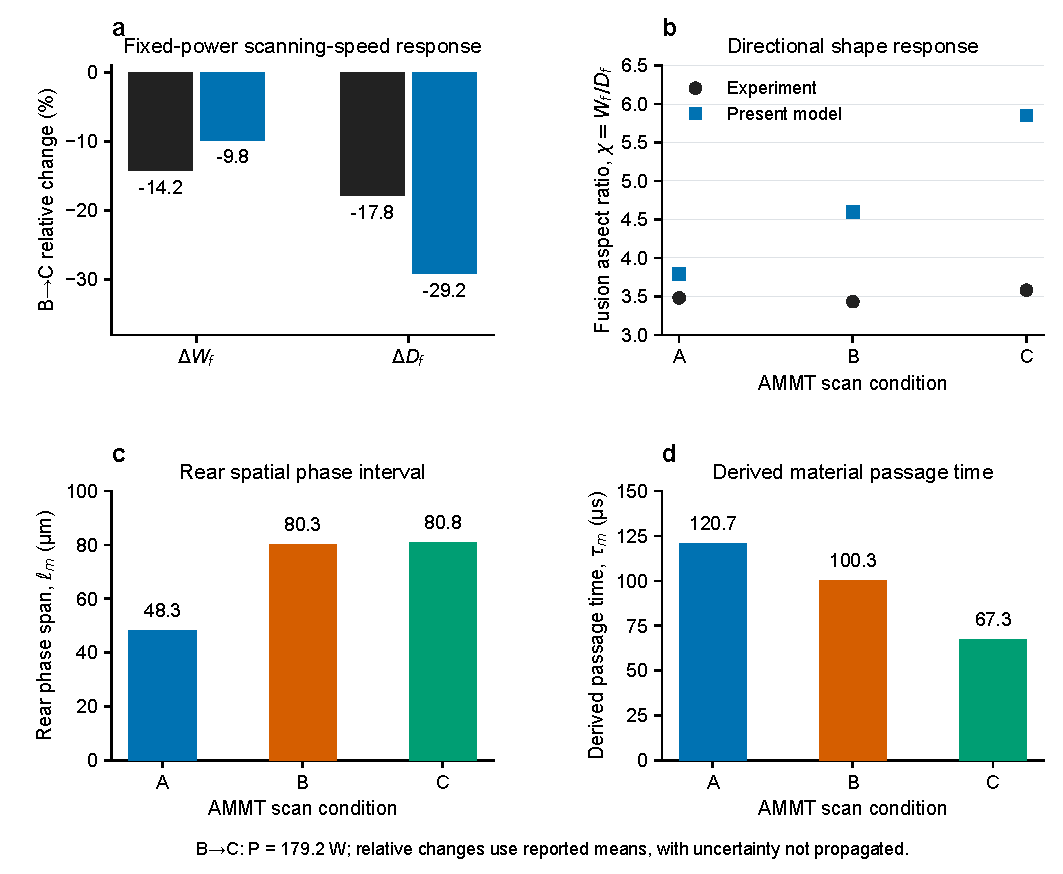
\includegraphics[width=\textwidth]{figures/ammt-research-condition-trends.pdf}
\caption{Operating-condition response. (a) Nominal B-to-C percentage changes in width and depth at fixed power, comparing model and condition-level reference means; uncertainty is not propagated. (b) Model and reference class-mean aspect ratios. (c) Model rear liquidus-to-solidus spatial spans. (d) Derived material passage times. The model histories share one steady solution and should not be counted as independent validation observables. Interval-mean cooling rates discussed in the text are derived over 1350--1290~$^\circ$C; they are not plotted here.}
\label{fig:trends}
\end{figure}

The operating-condition comparison therefore separates a change in the modeled fusion shape from a change in material passage time. The latter follows from the rear thresholds and speed; its experimental counterpart is not included in the geometric comparisons.

\subsection{Conductivity and storage continuations produce opposing tail responses}
The four-corner results are shown in Table~\ref{tab:factorial} and Fig.~\ref{fig:factorial}. Holding conductivity at its last table value increases length from 359.16 to 402.37~\um\ at linearly continued $c_p$. Holding $c_p$ instead decreases length to 352.99~\um. Holding both yields 393.44~\um. The joint increase is therefore
\begin{equation}
 \Delta L_{\rm joint}=43.21-6.17-2.76=34.28~\um.
\end{equation}
The heat-capacity response and interaction offset part of the conductivity response. A comparison of LL and HH alone would miss this decomposition. The signs persist at the other factor level: conductivity holding increases length by 40.45~\um{} when $c_p$ is held, and storage holding decreases length by 8.93~\um{} when $k$ is held. Conductivity therefore extends the tail and storage holding shortens it in both tested settings, with the interaction changing the magnitudes.

\begin{table}[htbp]
\centering
\caption{Fixed-B deterministic continuation contrast. The first letter labels $k$, the second $c_p$; L means linear continuation and H last-value holding above the respective endpoints. No branch is recalibrated. Rounded geometry and effects are in \um. Small transverse effects lack branch-specific refinement evidence.}
\label{tab:factorial}
\begin{tabular}{lrrr}
\toprule
Corner or contrast & $L$ & $W$ & $D$\\
\midrule
LL & 359.16 & 143.04 & 31.12\\
HL & 402.37 & 143.15 & 30.09\\
LH & 352.99 & 143.72 & 31.61\\
HH & 393.44 & 143.79 & 30.80\\
\midrule
$\delta_k$ & +43.21 & +0.11 & $-1.03$\\
$\delta_{c_p}$ & $-6.17$ & +0.68 & +0.49\\
$I_{k,c_p}$ & $-2.76$ & $-0.04$ & +0.21\\
$\Delta_{\rm joint}$ & +34.28 & +0.75 & $-0.32$\\
\bottomrule
\end{tabular}
\end{table}

Conductivity holding moves the rear solidus and liquidus by $-42.49$ and $-43.50$~\um, while the front solidus moves by +0.73~\um. The rear solidus displacement accounts for 98.3\% of the conductivity-induced length increase; the front contributes the remaining 1.7\%. The rear phase span changes by only $-1.01$~\um. Heat-capacity holding moves the rear positions forward by +6.22 and +6.53~\um, changing their separation by +0.31~\um. The large length response thus predominantly translates both rear phase boundaries together. It does not represent comparable broadening of the mushy interval.

At 1320~$^\circ$C, conductivity changes from 32.51 to 25.20~\si{\watt\per\metre\per\kelvin} under holding, a reduction of 22.48\%. Sensible specific heat decreases from 721.13 to 670~\si{\joule\per\kilogram\per\kelvin}, or 7.09\%. With the latent contribution included, effective specific heat decreases from 5387.79 to 5336.67~\si{\joule\per\kilogram\per\kelvin}, or 0.95\%, and enthalpy from the cold reference decreases by 0.66\%. This matched-temperature comparison describes the adopted mushy interval. A retained local face P\'eclet diagnostic for the mushy $\xi$ faces increases in median from 4.44 in LL to 5.77 in HL, consistent with reduced diffusion relative to coordinate enthalpy transport. The diagnostic is consistent with a conductivity-dependent shift in the model's transport balance. The corresponding retained rear hot-region outward diffusive flux rises from 14.724 to 14.913~W. Since that region is selected by temperature and changes with the solved state, conductivity holding cannot be equated with a measured reduction in its integrated outward heat flow. The branch also changes surface recovery consistently with $k$.

The current-mesh depth contrast illustrates cancellation. Conductivity holding changes it by $-1.03$~\um; heat-capacity holding contributes +0.49~\um\ and the interaction +0.21~\um, leaving a net $-0.32$~\um. All corners remain wider and shallower than the B reference. The conductivity depth effects remain negative at both storage levels ($-1.03$ and $-0.82$~\um), whereas the storage depth effects remain positive at both conductivity levels (+0.49 and +0.71~\um). These two continuation options therefore do not repair the baseline shape discrepancy. The main 34--43~\um\ length response substantially exceeds the retained baseline axial sensitivity; the 0.04~\um\ width interaction has no corresponding precision demonstration and is not interpreted as a robust fine ranking.

\begin{figure}[htbp]
\centering
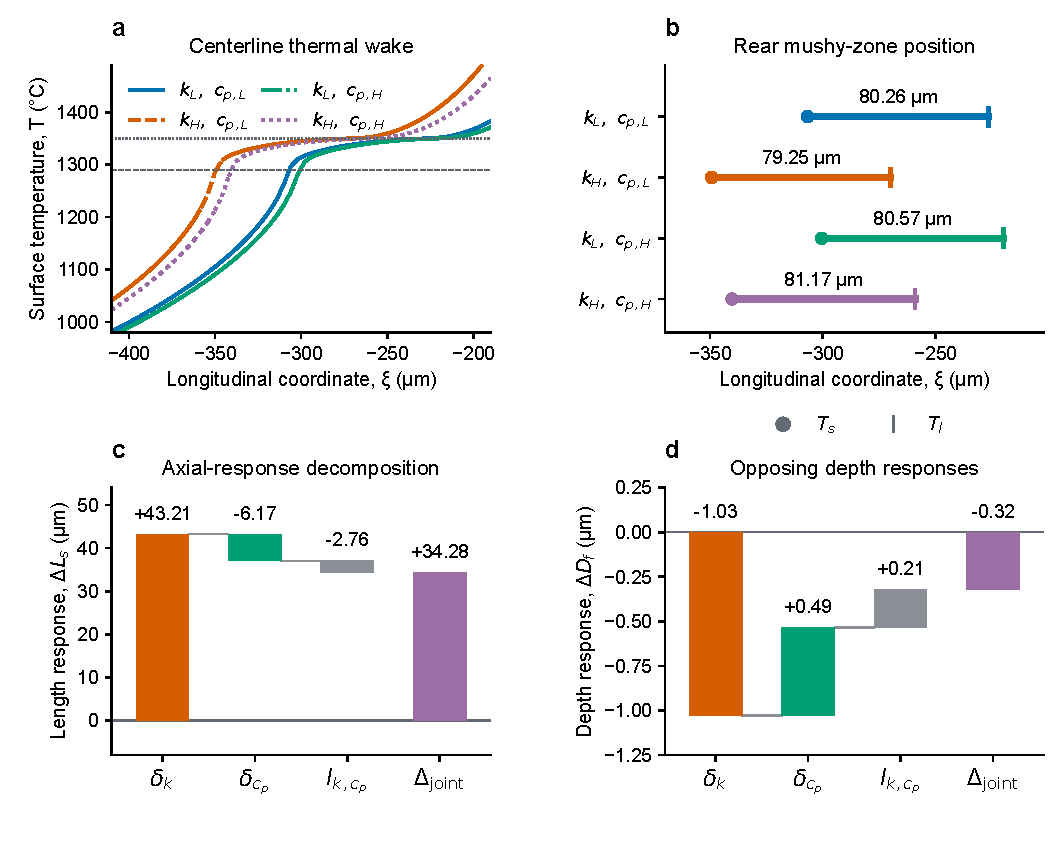
\includegraphics[width=\textwidth]{figures/ammt-research-constitutive-factorial.pdf}
\caption{Four-corner continuation comparison at fixed B: rear centerline temperature profiles, phase-boundary positions and spatial span, and baseline-anchored geometry effects. The same phase thresholds, source factor and mesh are retained. Profiles are plotted from original field values with segment clipping to the displayed window. Factorial effects are deterministic finite contrasts, not statistical effect estimates. Large rear translation dominates the length response; joint depth change conceals opposing single-factor contributions.}
\label{fig:factorial}
\end{figure}

Across the four corners, the rear phase span lies between 79.25 and 81.17~\um{} while total length ranges from 352.99 to 402.37~\um. The contrast consequently changes the location of the rear phase interval much more than its spatial separation. This is the main comparison supplied by the retained centerline profiles; the small span ordering remains a current-mesh result.

